\chapter{مقدمه}
\noindent
\textbf{
	\textit{
		توضیحی اولیه مبنی بر تعریف کلی فشرده‌سازی، انواع الگوریتم‌ها و کاربردها
	}
}
\pagenumbering{arabic}
\pagebreak
\section{تعریف}

الگوریتم‌های فشرده‌سازی، الگوریتم‌هایی هستند که می‌توان با استفاده از آن‌ها داده‌ها را طوری رمزنگاری کرد که در تعداد 	کمتری بیت\efn{Bit} نسبت به آرایش اولیه
قابل ارائه باشند\cite{data_compression}.
برای مثال می‌دانیم که برای ذخیرهٔ هر بیت اسکی
\efn{ASCII}
 هشت بیت فضا لازم است، می‌توان با استفاده از نگاشتی متشکل از حروف استفاده‌شده در 
یک متن تعداد بیت‌های مورد نیاز برای نشان دادن هر حرف استفاده‌شده در متن را کاهش داد.
با استفاده از این تکنیک در حقیقت متن را در قالب جدیدی فشرده کرده‌ایم.

\section{انواع الگوریتم‌های فشرده‌سازی}

در یک دسته‌بندی الگوریتم‌های فشرده‌سازی را به دو نوع زیر افراز می‌کنند:
\begin{itemize}
	\item  بدون هدررفت داده \efn{Lossless}
	\item  همراه با هدررفت داده \efn{Lossy}
\end{itemize}

\subsection{الگوریتم‌های بدون هدررفت داده}
در این سری الگوریتم‌ها دادهٔ ورودی بدون هیچ‌گونه هدررفتی از دادهٔ خروجی قابل بازیابی‌ست، الگوریتم‌های 
این دسته با استفاده از افزونگی آماری تلاش می‌کنند تا نحوهٔ نمایش داده را در نگاشتی به نحوهٔ نمایش دیگری که به فضای کمتری نیاز دارد 
تبدیل کنند.
این الگوریتم‌ها در مواقعی که 
ثابت ماندن داده در طی فشرده‌سازی الزامی‌ست استفاده می‌شوند، همچنین معمولا برای بازیابی اطلاعات فشرده‌شده نیاز به 
داده‌هایی خارجی است که با کمک آن عمل بازیابی انجام می‌گیرد، از این رو می‌توان از این نوع الگوریتم‌ها در رمزنگاری نیز 
استفاده کرد. یکی از کاربردهای اصلی این الگوریتم‌ها در فشرده‌سازی متون است که اشتباه شدن حتی یک حرف می‌تواند باعث بدخوانی و 
بدفهمی متن اصلی گردد. الگوریتم‌های مشهور فشرده‌سازی بدون هدررفت داده به شرح زیراند \cite{data_types}.

\begin{itemize}
	\item کدبندی طول اجرا\efn{\lr{Run-Length Enconding (RLE)}}
	\item فشرده‌سازی LZ\efn{\lr{Lempel-Ziv (LZ)}}
	\item کدگذاری هافمن\efn{\lr{Huffman Encoding}}
	\item تبدیل باروس-ویلر\efn{\lr{Burrows Wheeler Transform}}
\end{itemize}

البته لازم به ذکر است که در عمل از مجموعه‌ای از الگوریتم‌های فوق برای رسیدن به درصد مطلوب فشرده‌سازی استفاده می‌شود.
%todo: add my Compression project link to this section. 

\subsubsection{نمونه‌های الگوریتم‌های بدون هدررفت داده}
در عمل از الگوریتم‌های بدون هدررفت داده در مواقعی که 
پایداری داده‌های ذخیره‌شده حیاتی‌ست یا این که فایل در آینده به تعداد زیادی بار فشرده و گسترده می‌شود و از دست دادن قسمتی از داده در
هربار فشرده‌سازی منجر به اختلاف فاحش نهایی خواهد شد استفاده می‌شود. احتمالاً می‌توان مشهورترین فرمت فشرده‌سازی بدون هدررفت داده را
فرمت 
ZIP
نامید، این فرمت که برای فشرده‌سازی فایل‌های مختلف استفاده می‌شود به علت گستردگی استفاده در درون خود از 
الگوریتم‌های بدون هدررفت داده استفاده می‌کند، به جز فرمت ZIP 
فرمت‌های دیگری که استفاده‌های تخصصی‌تری دارند نیز از این الگوریتم‌ها استفاده می‌کنند که در ادامه به دو مورد مهم ایشان اشاره می‌کنیم.

\begin{itemize}
	\item \lr{PNG}\\
	در طراحی فرمت PNG برای فشرده‌سازی تصاویر از الگوریتم
	\lr{LZW}\efn{Lempel-Ziv-Welch}
	که الگوریتی بدون هدررفت داده است استفاده شده. 
	در 
	شکل 	\ref{example_1} و 
	جدول 	\ref{compare_1} 
	یک نمونه عکس در حالت فشرده‌نشده و فشرده‌شده با فرمت PNG
	و مقدار حجم آن در حالت‌های مختلف آورده شده است.

	\item کدک صوتی بدون هدررفت دادهٔ آزاد \cite{flac}\\
	کدک صوتی بدون هدررفت دادهٔ آزاد \efn{\lr{Free Lossless Audio Codec}} یا FLAC
	الگوریتمی که با استفاده از اطلاعات ذاتی داده‌های صوتی به فشرده‌سازی آن‌ها می‌پردازد، نرخ فشرده‌سازی این الگوریتم با توجه به 
	سطح فشرده‌سازی آن معمولا بین ۴۰ تا ۶۰ درصد می‌باشد اما در حالت بیشینه ممکن است تا ۸۰ درصد هم برسد.
	
\end{itemize}

\begin{figure}[H]
	\centering
	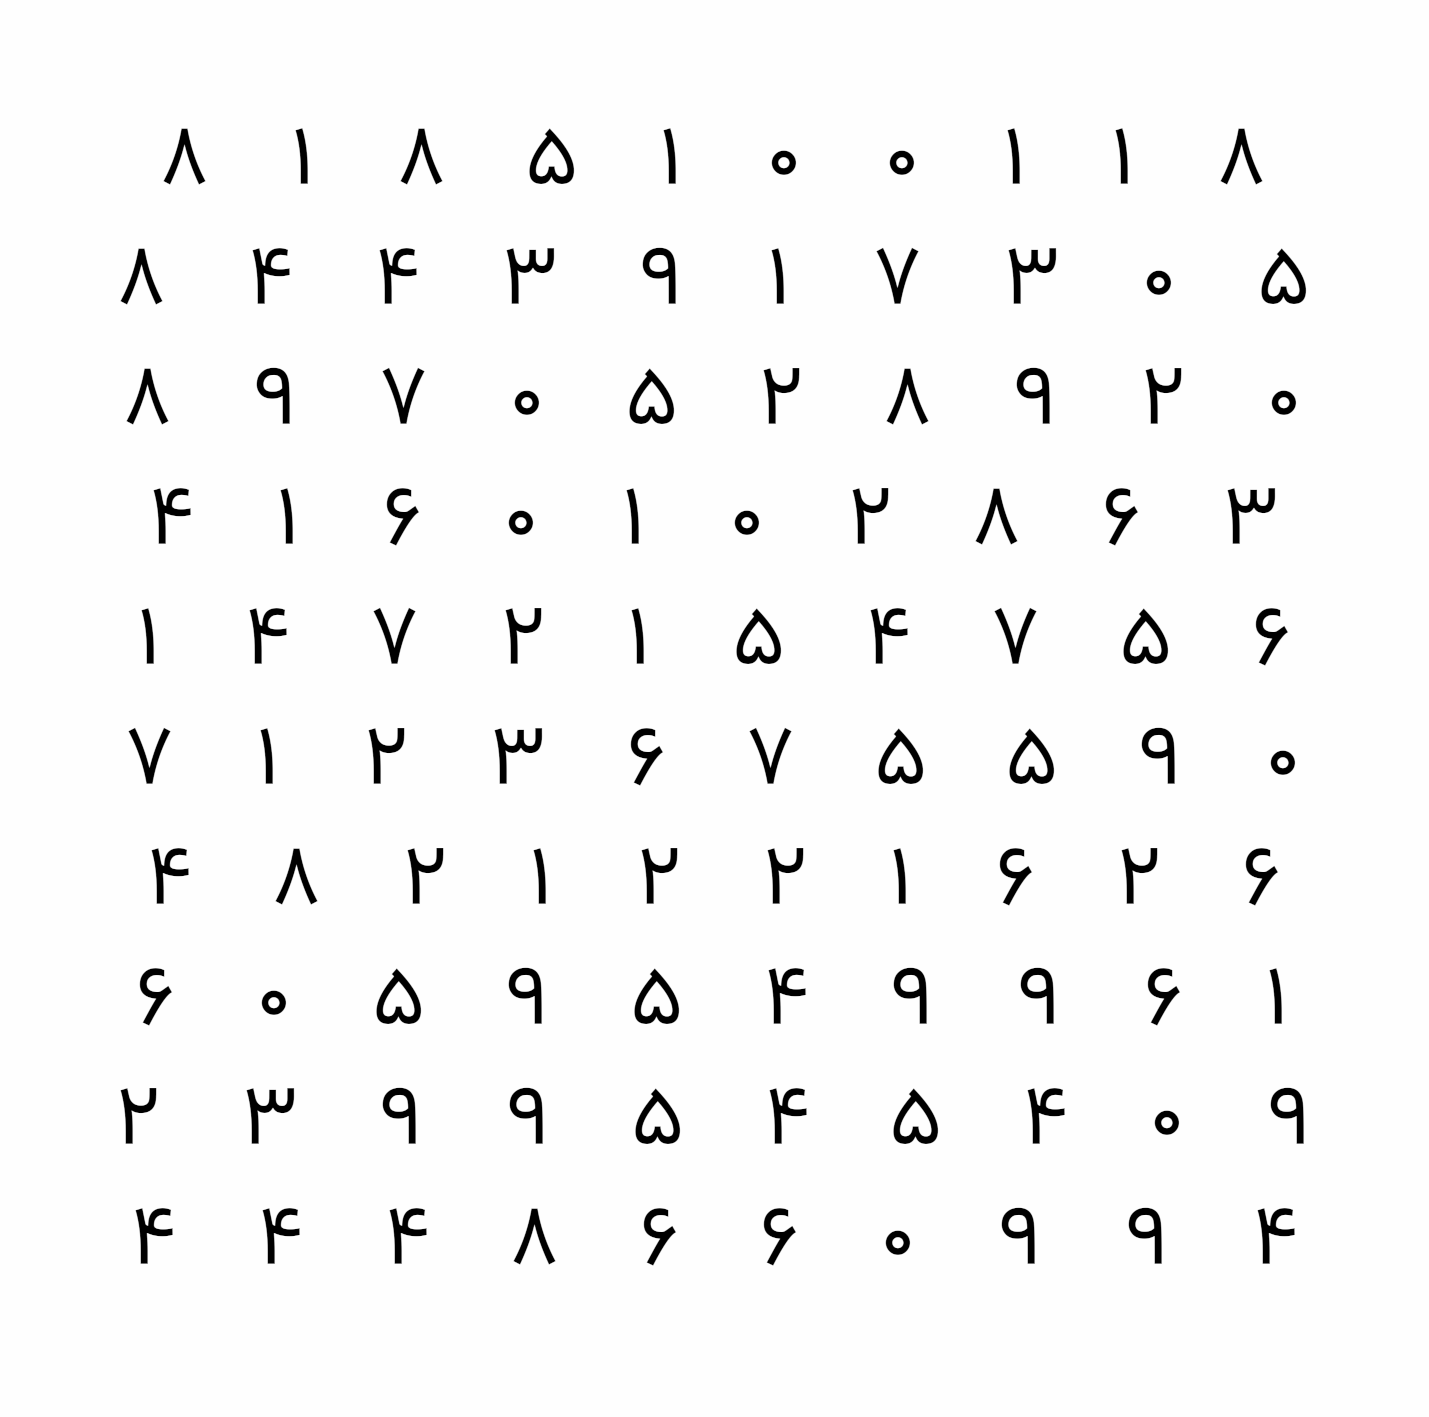
\includegraphics[scale=0.6]{figs/compressed.png}
	\caption[شکل نمونه برای تست میزان فشرده‌سازی در فرمت PNG ]{شکل نمونه برای تست میزان فشرده‌سازی در فرمت PNG \cite{my_picture}}
	\label{example_1}
\end{figure}

\begin{table}[H]
	\centering
	\caption{حجم فایل نمونه در فرمت PNG }
	\label{compare_1}
	\begin{tabular}{@{}ll@{}}
	\toprule
	اندازه & فرمت \\ \midrule
	7.7 مگابایت & BMP \\
	98 کیلوبایت & PNG \\ \bottomrule
	\end{tabular}
\end{table}



\subsection{الگوریتم‌های با هدررفت داده}

معمولا در فشرده‌سازی با هدررفت داده از تبدیل‌‌ فضایی 
\efn{\lr{Transformation}}
استفاده می‌شود که داده‌ها را از فضای حقیقی به فضایی دیگر(معمولا فرکانس) می‌برد و در آنجا از قسمت‌هایی از داده که تاثیرگذاری و حس‌پذیری کمتری
نسبت به دیگران دارند صرف نظر می‌شود، سپس وارون تبدیل اجرا شده و داده‌های کوچک‌شدهٔ جدید این بار با الگوریتم‌های 
بدون هدررفت داده فشرده می‌شوند. یکی از 
مشهورترین
تبدیل‌های فضایی
ها تبدیل کسینوسی گسسته
\efn{Discrete Cosine Transform (DCT)}
است که در فصل‌ دوم این مستند بیشتر با آن آشنا خواهیم شد
\cite{dct}.
\subsubsection{نمونه‌های الگوریتم‌های با هدررفت داده}
الگوریتم‌های با هدررفت داده با همه‌گیر شدن اینترنت و اشتراک‌گذاری 
بیشتر محتوای رسانه‌ای در فضای اینترنت بسیار گسترده شدند، از این رو اکثر این الگوریتم‌ها برای فشرده‌سازی فایل‌های صوتی-تصویری یا به اصطلاح 
مدیا\efn{Media}
استفاده می‌شوند. فرمت‌های زیر همگی در بطن خود از الگوریتم‌های با هدررفت داده برای فشرده‌سازی مدیا استفاده می‌کنند.

\begin{itemize}
	\item JPEG
	\item \lr{MP3}
	\item \lr{MP4}
	\item \lr{H.26x}
\end{itemize}
به عنوان نمونهٔ برای الگوریتم باهدررفت داده 
حالت فشرده‌شدهٔ عکس 
\ref{example_1}
با فرمت JPEG 
با کیفیت‌های مختلف در جدول 
\ref{compare_2}
آورده شده است.
% \footnote{در صورتی که تمایل به دیدن اصل فایل‌ها دارید می‌توانید به 
% \textit{  \href{https://github.com/merfanian/DataCompressionDoc/tree/master/LatexFiles/figs}{Github مستند} 
% } 
% مراجعه کنید.
% } 

\begin{table}[h]
	\centering
	\caption{حجم فایل نمونه در فرمت JPG}
	\label{compare_2}
	\begin{tabular}{@{}lll@{}}
	\toprule
	کیفیت(\%) & اندازه & فرمت \\ \midrule
	100 & 7.7 مگابایت & BMP \\
	100 & 98 کیلوبایت & PNG \\
	90 & 96.8 کیلوبایت & JPG \\
	50 & 62.9 کیلوبایت & JPG \\
	20 & 49  کیلوبایت& JPG \\ \bottomrule
	\end{tabular}
	\end{table}


\section{کاربردهای دیگر فشرده‌سازی}
الگوریتم‌های فشرده‌سازی داده علاوه بر این که در کاربرد اصلی خود یعنی فشرده کردن فایل‌ها بسیار استفاده می‌شوند اما کاربردهایی دیگری هم در دنیای
کامپیوتر دارند، به عنوان مثال یکی از حیاتی‌ترین عناصر پردازش سیگنال\efn{\lr{Signal Processing}} 
را فشرده‌سازی سیگنال تشکیل می‌دهد. در ارتباطات رادیویی برای بالا بردن امنیت و کم کردن هزینهٔ انتقال از فشرده‌سازی داده استفاده می‌شود. 

از دیگر کاربردهای جدید فشرده‌سازی داده ژنتیک است، رشته‌های دی‌ان‌ای\efn{DNA}
و آر‌ان‌ای\efn{RNA}
 را معمولا می‌توان به صورت
یک رشته متنی نشان داد و با الگوریتم‌های فعلی فشرده‌سازی متن فشرده کرد اما به دلیل این که این رشته‌ها طول و تعداد زیادی دارند
بهتر است از روش‌های دیگری برای بازیابی و فشرده‌سازی سریع آن‌ها استفاده کنیم، با رشد سریع ژنتیک و بایوانفورماتیک در جهان و نیاز
مبرم به ذخیره‌سازی رشته‌های دی‌ان‌ای و آران‌ای 
الگوریتم‌های مختلفی مختص فشرده‌سازی این رشته‌ها معرفی شده اند\cite{dna}. 